%% bare_jrnl.tex
%% V1.3
%% 2007/01/11
%% by Michael Shell
%% see http://www.michaelshell.org/
%% for current contact information.
%%
%% This is a skeleton file demonstrating the use of IEEEtran.cls
%% (requires IEEEtran.cls version 1.7 or later) with an IEEE journal paper.
%%
%% Support sites:
%% http://www.michaelshell.org/tex/ieeetran/
%% http://www.ctan.org/tex-archive/macros/latex/contrib/IEEEtran/
%% and
%% http://www.ieee.org/

%%*************************************************************************
%% Legal Notice:
%% This code is offered as-is without any warranty either expressed or
%% implied; without even the implied warranty of MERCHANTABILITY or
%% FITNESS FOR A PARTICULAR PURPOSE!
%% User assumes all risk.
%% In no event shall IEEE or any contributor to this code be liable for
%% any damages or losses, including, but not limited to, incidental,
%% consequential, or any other damages, resulting from the use or misuse
%% of any information contained here.
%%
%% All comments are the opinions of their respective authors and are not
%% necessarily endorsed by the IEEE.
%%
%% This work is distributed under the LaTeX Project Public License (LPPL)
%% ( http://www.latex-project.org/ ) version 1.3, and may be freely used,
%% distributed and modified. A copy of the LPPL, version 1.3, is included
%% in the base LaTeX documentation of all distributions of LaTeX released
%% 2003/12/01 or later.
%% Retain all contribution notices and credits.
%% ** Modified files should be clearly indicated as such, including  **
%% ** renaming them and changing author support contact information. **
%%
%% File list of work: IEEEtran.cls, IEEEtran_HOWTO.pdf, bare_adv.tex,
%%                    bare_conf.tex, bare_jrnl.tex, bare_jrnl_compsoc.tex
%%*************************************************************************

\documentclass[journal]{IEEEtran}

\newcommand{\subparagraph}{}
\def\naive{na\"{\i}ve}

\usepackage{amsmath,
            amssymb,
            amsthm,
            atbegshi,
            caption,
            subcaption,
            epigraph,
            etoolbox,
            enumitem,
            fancyhdr,
            geometry,
            graphicx,
            hyperref,
            kpfonts,
            lipsum,
            longtable,
            natbib,
            tabulary,
            thmtools,
            tikz,
            tikzpagenodes,
            titletoc,
            titlesec,
            tocloft,
            url,
            wrapfig
}
\usepackage[utf8]{inputenc}
\usetikzlibrary{arrows}

\tikzset{%
    treenode/.style = {align=center, inner sep=0pt, text centered,
    font=\sffamily},
    arn_n/.style = {treenode, circle, white, font=\sffamily\bfseries,
    draw=black, fill=black, text width=1.5em},% arbre rouge noir, noeud noir
    arn_r/.style = {treenode, circle, red, draw=red,
    text width=2.9em, very thick},% arbre rouge noir, noeud rouge
    arn_x/.style = {treenode, rectangle, draw=black,
    minimum width=0.5em, minimum height=0.5em}% arbre rouge noir, nil
}

\begin{document}
%
% paper title
% can use linebreaks \\ within to get better formatting as desired
\title{2048 Expectimax Solver}

\author{Anders Sildnes, Andrej Leitner~\IEEEmembership{students of NTNU}% <-this % stops a space. jobtitle in memberkj
}% \thanks{Utsendt 2014}}

% The paper headers
\markboth{2048 Expectimax Solver}%
{h}

% make the title area
\maketitle

\begin{abstract}
    This text answers assignment 5: writing a solver for the game 2048.
    The purpose of the game is to slide tiles with numbers $2^{n}$, and join them
    together to form 2048 ($2^{11}$), or possibly higher.
    We present a solver using Expectimax algorithm. We explain our choice of
    heuristics and results.
\end{abstract}

% \begin{IEEEkeywords}
%     Stuff
% \end{IEEEkeywords}
\IEEEPARstart{2}{048} can be thought of as a 2-player, turn-based game. The
opponent places tiles valued either $2$ or $4$ in an availible location. Then,
the other player makes a move to slide all tiles in a given direction. This
goes back and forth until there are no more availible moves.

In a turn-based game, you have the time to consider the consequences for each possible
action. This gives computers immense advantages over humans:
IBM's chess-solving machine ``Deep Blue'' won against Garry Kasparov in 1997 considered more than
200 million possible moves per second\footnote{For more, see
    \href{http://www-03.ibm.com/ibm/history/ibm100/us/en/icons/deepblue/}
{http://www-03.ibm.com/ibm/history/ibm100/us/en/icons/deepblue/}}.
In the case of 2048, this could yield a valid solution in a short amount of
time. However, not everyone has access to such fast hardware and
multi-threading so a way to prune the search space is needed.

\section*{Assumptions}
While we yearn to learn and explore science, time is a serious impendiment.
Therefore we have rigiously worked to create a solver within the assignment bounds:
\begin{enumerate}
    \item The highest value tile does not need to exceed 4096.
    \item Execution time is not critical (roughly $< 10$minutes)
\end{enumerate}
This implies that our chosen heuristic and solver method does not need a strong
level of optimization to work. Indeed, the work of~\cite{brutesolver} shows that
a \naive{} brute force can be used to solve the game within the bounds listed above.

\section*{Minimax Algorithm}
The purpose of minimax is to minimize loss for a worst possible scenario.
This means choosing an action such that your opponent can do ``least amount of damages'',
i.e.\ leaving you in a promising state. This is also called \textit{adversial search}.
For 2048 this would mean always making a move such that no matter where the next
tile goes, and no matter what value, you will still find a way for success.

% PERFECT INFORMATION
% DISCRETE SPACE
% PLY

2048, however, is a stochastic game. The opponent will never purposly select a
bad tile, nor \textit{choose} a bad value. This is to say that there is no opponent,
so it is possible to always land a best case scenario. Therefore, we felt that minimax,
considering the worst case, is too pessimistic in its search space.
Furthermore, the distribution of numbered tiles are given:
there is a 90\% chance of getting a tile valued 2, and 10\% chance of getting a tile
valued 4. The location is random. Also note that in some cases, a tile
in position $i,j$  is no different from having a tile in position $i+i,j$ if the
next move it to slide the tiles downward. Thus the possible search space
is not too big and one can use statistics to get accurate enough resuls.


Using stochastic information in adversial search leads to expectimax.
After expanding the search space up to a given depth, you can back up from each
node and introduce a chance node. The chance nodes multiply the value to each
of its children (given a state, the objective value to each of the children).
The chance nodes are used when pruning the search space. Their importance is that
unlikely values will yield a lower penalty to the overall score of the search node,
such that the node is not necessarily pruned away.

\section*{Heuristic}
To assess whether or not a current game state is good or not, we have different
objective functions to assess game state. Using these to advance in the
solution space is called heuristical search. Our heuristics are developed based
on ideas we found online and through some play of our own.
BENCHMARK
BENCHMARK
BENCHMARK
BENCHMARK
BENCHMARK
BENCHMARK
BENCHMARK
BENCHMARK
\subsection*{Gradients}
If a large value is in the middle of the board, it will be hard to pair up
with other adjacent tiles. Therefore, we would like to set a natural preference
for having larger values clustered in a corner. This way, they do not interfere
with other lower-valued tiles. Next to the highest value tile, you want other,
lower valued cells. This extends throughout the board. However, having large values
in two corners implies that we have two (or more) tiles with large values, separated
by lower tiles. Therefore, we penalize boards where large values are far apart.

To calculate the value of a board, we apply a $4\times{}4$ mask and retrieve the
sum of adding all the values in the masked board.
The mask is shown \autoref{fig:gradient}. Each number in the tiles represents a scalar
which is multiplied with the value from the board. Since large value might be clustered
in all corners, we apply 4 masks, one for each corner respectively. Then,
the largest resulting value is chosen as the one to be used as a value for the state.

\begin{figure}[Hb]
\centering
  % TikZ picture with origin upper left
    \begin{tikzpicture}[yscale=-1]
        % 4x4 grid
        \draw (0, 0) grid (4, 4);
        % origin point
        % \draw [color=blue, fill=blue] (0, 0) circle (0.1);
        % % x-axis
        % \draw [thick,->] (0, 0) -- (3.5, 0);
        % % y-axis
        % \draw [thick,->] (0, 0) -- (0, 3.5);
        % origin label
        % \node at (-0.5, 0.5) {1};
        \node at (0.5, 0.5) {3};
        \node at (1.5, 0.5) {2};
        \node at (2.5, 0.5) {1};
        \node at (3.5, 0.5) {0};

        \node at (0.5, 1.5) {2};
        \node at (1.5, 1.5) {1};
        \node at (2.5, 1.5) {0};
        \node at (3.5, 1.5) {-1};

        \node at (0.5, 2.5) {1};
        \node at (1.5, 2.5) {0};
        \node at (2.5, 2.5) {-1};
        \node at (3.5, 2.5) {-2};

        \node at (0.5, 3.5) {0};
        \node at (1.5, 3.5) {-1};
        \node at (2.5, 3.5) {-2};
        \node at (3.5, 3.5) {-3};
        % % x-axis label
        % \node at (4.5, -0.5) {200px};
        % % y-axis label
        % \node at (0, 5) {200px};
    \end{tikzpicture}
    \caption{Our gradient mask}
\label{fig:gradient}
\end{figure}

\section*{Why not use more heuristics?}

Many other heuristic functions exist:
\begin{enumerate}
    \item\label{it:score} \textbf{Board score} \textendash{} whenever two cells merge, the board score increases.
    \item\label{it:free} \textbf{Free tiles} \textendash{} giving scores based on how many cells are left.
    \item\label{it:nonmono} \textbf{Non-monotnic rows/coumns} \textendash{} prefer boards where there are large, but similar
        tiles.
    \item\label{it:merges} \textbf{Possible merges} \textendash{} prefer boards where many merges are possible,
       i.e.\ boards with tiles of the same value.
\end{enumerate}

Heuristic~\ref{it:score} is difficult to implement in practise. When greedily preffering
boards with higher tiles you might exclude boards with high merges.
Heuristic~\ref{it:free} can also be used. Arguably, it is already used in our gradient
function: boards with tiles in opposite corners are penalized. Therefore we did
not see the need to implement this heuristic expliclitly. Furthermore, there are
cases where having many free tiles not necessarily is a bad thing.
The two last heuristics are shown to

Exepctimax has execution time $O(b^{m}n^{m})$. Here, $b$ is the \textit{branching factor},
i.e.\ the number of possible children from a given board. For each state, $0
\leq b \leq 4$.  $m$ is the depth of the search tree. $n$ is the number of possible
moves, i.e.\ possible tiles with value either $2$ or $4$. It can easily be seen
that this execution time quickly grows: for a search depth of 6, the execution
time is $4^{6}\cdot{n^{4}}$ for each possible move. In addition, we have to apply our mask
in~\autoref{fig:gradient} four times and introduce chance nodes. Therefore, to
avoid cluttered code and execution, we chose to only rely on the gradient
method. However, if this assignment had rewarded execution time and scores
higher than $4096$, we would implement more of the heuristics mentioned above.

\section*{Structure of source code}
We implemented our solution in Java. This is because both members of the group
were familiar with the language. The GUI is rendered through a JFrame, and the tiles are
drawn using AWT's Graphics2D.

There is a builtin keylistener that reads for keyboard input. However, one can also
enable autosolving, which toggles a flag in the keylistener and solves the board by
itself. The builtin solver works as follows:
\begin{enumerate}
    \item For each possible move (left,right,up,down) by the player, call ``computers''
    \item ``computer'': For each possible tile placement:
        \begin{enumerate}
            \item place a tile
            \item call all possible player moves,
                decrementing depth by 1
        \end{enumerate}
    \item calculate E[current state]
    \item \dotso{} goto step 1 if depth \textgreater{} 0
    \item Get E[current node], multiply upward to root
    \item Once complete $k$-depth=tree is complete, choost most promising branch.
\end{enumerate}

\begin{figure}[Hb!]
\begin{tikzpicture}[->,>=stealth',level/.style={sibling distance = 4cm/#1,
  level distance = 1.5cm}]
  \node [arn_n, label={[label distance=.2cm]20:current board}] {}
  child{node [arn_r,label={[label distance=0.4cm]20:possible tiles\dotso{}}] {$15\cdot{p_{a}}$}
            % 
            child{node [arn_n] {16} edge from parent node[above left] {N} }
            child{node [arn_n] {20} edge from parent node[above left] {S} }
            child{node [arn_n] {30} edge from parent node[above right] {W} }
    }
    child{node [arn_r] {$47\cdot{p_{b}}$}
            child{node [arn_n] {15} edge from parent node[above left] {N} }
            child{node [arn_n] {09} edge from parent node[above left] {E} }
        }
;
\end{tikzpicture}
\caption{Example expectimax tree, with implicit chance nodes}
\end{figure}

To realize the above code, a few classes are needed. We implemented each 
possible board as a class with each tile as a subclass. It could be noted that since each tile will not need
to exceed $2^16 = 65536$, a 64 bit architecture can represent one row as a 64-bit number
($16 \times 4$) which permits fast bitwise operations for altering the board.
However, without classes (objects) the GUI is more difficult to render, so we 
chose not to use this apporach, even though it allows fast board checks.

\section*{Results}
Our highest result achieved so far is 8192. On average, we achieve $4096$ in 80\%
of the cases, in about XXX minutes. \autoref{fig:max} shows this result and
our board.

\begin{figure}[Hb]
\centering
    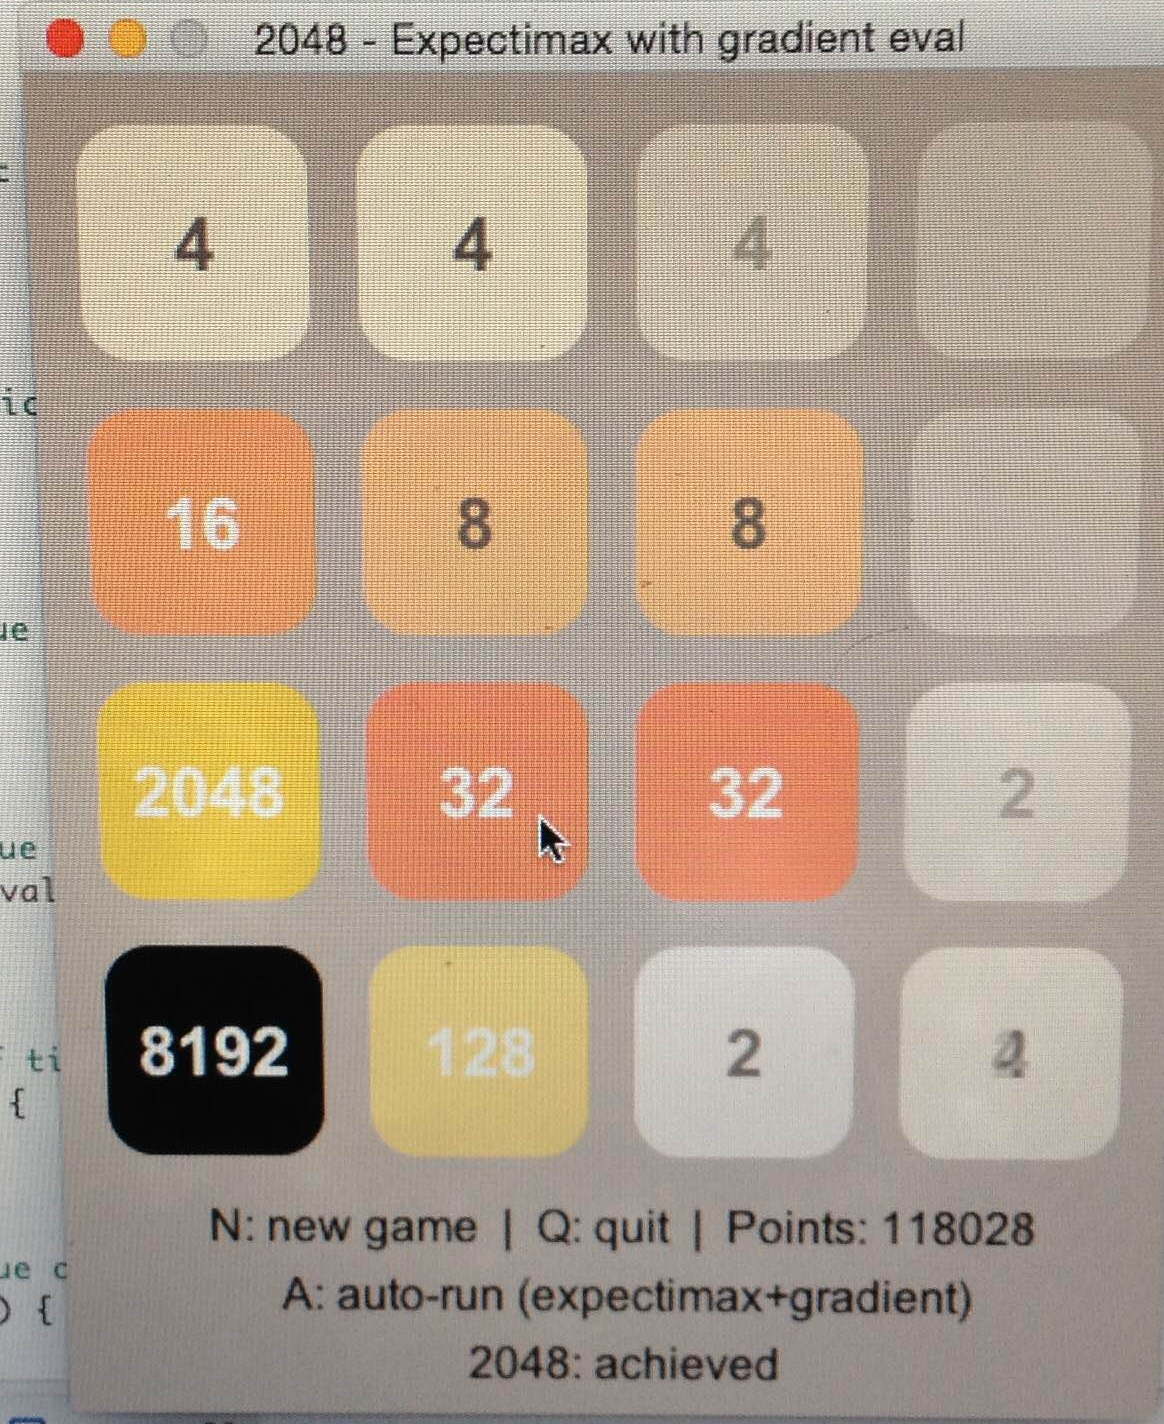
\includegraphics[keepaspectratio, height=3cm]{fig/8192.png}
\caption{Example solver and board}
\label{fig:max}
\end{figure}




\bibliographystyle{IEEEtran}
% \bibliography{IEEEabrv,../bib/paper}
\begin{thebibliography}{1}
\bibitem{brutesolver}
    ``ronzil'' \emph{2048-AI}, \textit{git-repository}.\hskip 1em plus
  0.5em minus 0.4em\relax GitHub
\end{thebibliography}

\end{document}
